\documentclass{beamer}

%\usepackage{verbatim}
\usepackage{anyfontsize}
\usepackage{tikz}
\usepackage{media9}
\usepackage{graphicx}

\usetheme{Boadilla}

\DeclareMathOperator*{\argmax}{argmax}
\DeclareMathOperator*{\argmin}{argmin}

\newcommand{\ba}{\ensuremath{\mathbf{a}}}
\newcommand{\bb}{\ensuremath{\mathbf{b}}}
\newcommand{\bx}{\ensuremath{\mathbf{x}}}
\newcommand{\bo}{\ensuremath{\mathbf{o}}}
\newcommand{\bC}{\ensuremath{\mathbf{C}}}
\newcommand{\bq}{\ensuremath{\mathbf{q}}}


\title{
    Whale Song Unit Classification
}
\subtitle{
    Some Preliminary Exploration\\
    Using Linear Prediction Vector Quantization\\
    and Hidden Markov Modeling
}
\author{Carlos Rueda}

\begin{document}

\frame {
    \titlepage
}

\frame {
    \frametitle{The Problem}

    Following Mitchell (1997), we state the problem as follows:

    \begin{itemize}
        \setlength\itemsep{1em}
        \item \alert{Task}: \\
            Classify whale song unit instances\\
            according to a given vocabulary of whale song unit types

        \item \alert{Performance measure}:\\
            Percent of instances correctly classified

        \item \alert{Training experience}:\\
            A database of labelled whale song unit instances
    \end{itemize}
}

\begin{frame}[fragile]
    \frametitle{Whale Song Units}

    \centering
    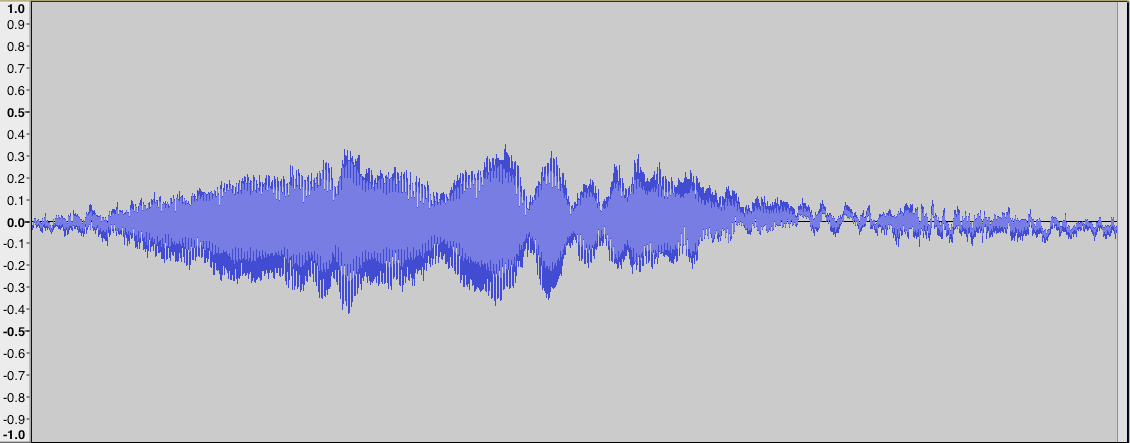
\includegraphics[width=0.7\textwidth]{from_HBSe_20151207T070326__124_45328_126_52461.png}
    \includemedia[
        height=0.44em,
        addresource=from_HBSe_20151207T070326__124.45328_126.52461.mp3,
        flashvars={
            source=from_HBSe_20151207T070326__124.45328_126.52461.mp3
            &autoPlay=true
        }
    ]{\fbox{Play}}{APlayer.swf}

    {\tiny A ``modulated cry'' instance, from \verb|HBSe_20151207T070326.wav, 124.5sec-126.5sec|}

    \begin{itemize}
        \setlength\itemsep{1em}
        \item
            Acoustic signal:
            \begin{equation*}
            \bx = \langle x_1, x_2, \ldots, x_N \rangle \qquad (N=66,283)
            \end{equation*}


    \end{itemize}
\end{frame}

\frame{
\frametitle{Linear Predictive Coding}

\begin{itemize}
    \setlength\itemsep{1em}
    \item
    Acoustic signal:
    \begin{equation*}
        \bx = \langle x_1, x_2, \ldots, x_N \rangle
    \end{equation*}

    \item
    Transformed into a sequence of \alert{predictor} vectors:
    \begin{equation*}
        \ba = \langle \ba_1, \ba_2, \ldots, \ba_T \rangle
    \end{equation*}

    \item
    Transformed into a \alert{sequence of symbols}:
    \begin{equation*}
        \bo = \langle o_1, o_2, \ldots, o_T \rangle
    \end{equation*}
    where $o_t \in \{ 1, 2, \ldots, M \}$

\end{itemize}

}

\frame{
\frametitle{Linear Predictive Coding}

\hspace*{0.77in}
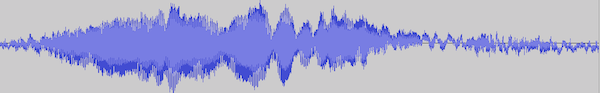
\includegraphics[width=0.77\textwidth]{from_HBSe_20151207T070326__124_45328_126_52461_small.png}

\tikzset{every picture/.style={line width=0.75pt}} %set default line width to 0.75pt

\begin{tikzpicture}[x=0.75pt,y=0.75pt,yscale=-1,xscale=1]
    %uncomment if require: \path (0,450); %set diagram left start at 0, and has height of 450

    %Straight Lines [id:da01594281834627176]
    \draw    (80.33,6.78) -- (346.26,6.78) (85.33,2.78) -- (85.33,10.78)(90.33,2.78) -- (90.33,10.78)(95.33,2.78) -- (95.33,10.78)(100.33,2.78) -- (100.33,10.78)(105.33,2.78) -- (105.33,10.78)(110.33,2.78) -- (110.33,10.78)(115.33,2.78) -- (115.33,10.78)(120.33,2.78) -- (120.33,10.78)(125.33,2.78) -- (125.33,10.78)(130.33,2.78) -- (130.33,10.78)(135.33,2.78) -- (135.33,10.78)(140.33,2.78) -- (140.33,10.78)(145.33,2.78) -- (145.33,10.78)(150.33,2.78) -- (150.33,10.78)(155.33,2.78) -- (155.33,10.78)(160.33,2.78) -- (160.33,10.78)(165.33,2.78) -- (165.33,10.78)(170.33,2.78) -- (170.33,10.78)(175.33,2.78) -- (175.33,10.78)(180.33,2.78) -- (180.33,10.78)(185.33,2.78) -- (185.33,10.78)(190.33,2.78) -- (190.33,10.78)(195.33,2.78) -- (195.33,10.78)(200.33,2.78) -- (200.33,10.78)(205.33,2.78) -- (205.33,10.78)(210.33,2.78) -- (210.33,10.78)(215.33,2.78) -- (215.33,10.78)(220.33,2.78) -- (220.33,10.78)(225.33,2.78) -- (225.33,10.78)(230.33,2.78) -- (230.33,10.78)(235.33,2.78) -- (235.33,10.78)(240.33,2.78) -- (240.33,10.78)(245.33,2.78) -- (245.33,10.78)(250.33,2.78) -- (250.33,10.78)(255.33,2.78) -- (255.33,10.78)(260.33,2.78) -- (260.33,10.78)(265.33,2.78) -- (265.33,10.78)(270.33,2.78) -- (270.33,10.78)(275.33,2.78) -- (275.33,10.78)(280.33,2.78) -- (280.33,10.78)(285.33,2.78) -- (285.33,10.78)(290.33,2.78) -- (290.33,10.78)(295.33,2.78) -- (295.33,10.78)(300.33,2.78) -- (300.33,10.78)(305.33,2.78) -- (305.33,10.78)(310.33,2.78) -- (310.33,10.78)(315.33,2.78) -- (315.33,10.78)(320.33,2.78) -- (320.33,10.78)(325.33,2.78) -- (325.33,10.78)(330.33,2.78) -- (330.33,10.78)(335.33,2.78) -- (335.33,10.78)(340.33,2.78) -- (340.33,10.78)(345.33,2.78) -- (345.33,10.78) ;


    %Shape: Grid [id:dp23348643338301867]
    \draw  [draw opacity=0] (91.83,60.78) -- (96.83,60.78) -- (96.83,85.78) -- (91.83,85.78) -- cycle ; \draw    ; \draw   (91.83,65.78) -- (96.83,65.78)(91.83,70.78) -- (96.83,70.78)(91.83,75.78) -- (96.83,75.78)(91.83,80.78) -- (96.83,80.78) ; \draw   (91.83,60.78) -- (96.83,60.78) -- (96.83,85.78) -- (91.83,85.78) -- cycle ;
    %Straight Lines [id:da18845328084567692]
    \draw    (83.96,23) -- (231.27,23) ;


    %Straight Lines [id:da22066749517532758]
    \draw    (83.96,23) -- (84.02,15.78) ;


    %Straight Lines [id:da17781894400268783]
    \draw    (231.27,23) -- (231.33,15.78) ;



    %Down Arrow [id:dp1641348319045337]
    \draw   (89.83,34.38) -- (91.87,34.38) -- (91.87,23) -- (95.96,23) -- (95.96,34.38) -- (98,34.38) -- (93.92,42.33) -- cycle ;
    %Shape: Grid [id:dp5596357312856071]
    \draw  [draw opacity=0] (155.83,60.78) -- (160.83,60.78) -- (160.83,85.78) -- (155.83,85.78) -- cycle ; \draw    ; \draw   (155.83,65.78) -- (160.83,65.78)(155.83,70.78) -- (160.83,70.78)(155.83,75.78) -- (160.83,75.78)(155.83,80.78) -- (160.83,80.78) ; \draw   (155.83,60.78) -- (160.83,60.78) -- (160.83,85.78) -- (155.83,85.78) -- cycle ;
    %Shape: Grid [id:dp23574651045711348]
    \draw  [draw opacity=0] (410.83,60.78) -- (415.83,60.78) -- (415.83,85.78) -- (410.83,85.78) -- cycle ; \draw    ; \draw   (410.83,65.78) -- (415.83,65.78)(410.83,70.78) -- (415.83,70.78)(410.83,75.78) -- (415.83,75.78)(410.83,80.78) -- (415.83,80.78) ; \draw   (410.83,60.78) -- (415.83,60.78) -- (415.83,85.78) -- (410.83,85.78) -- cycle ;
    %Straight Lines [id:da5803547653809475]
    \draw    (147.96,35) -- (295.27,35) ;


    %Straight Lines [id:da7303303253711202]
    \draw    (147.96,35) -- (148.02,27.78) ;


    %Straight Lines [id:da7587981770652479]
    \draw    (295.27,35) -- (295.33,27.78) ;



    %Down Arrow [id:dp8762704300541813]
    \draw   (153.83,46.38) -- (155.87,46.38) -- (155.87,35) -- (159.96,35) -- (159.96,46.38) -- (162,46.38) -- (157.92,54.33) -- cycle ;
    %Down Arrow [id:dp14503895036340997]
    \draw   (91.83,140.38) -- (93.87,140.38) -- (93.87,129) -- (97.96,129) -- (97.96,140.38) -- (100,140.38) -- (95.92,148.33) -- cycle ;
    %Down Arrow [id:dp3912637147310176]
    \draw   (154.83,140.38) -- (156.87,140.38) -- (156.87,129) -- (160.96,129) -- (160.96,140.38) -- (163,140.38) -- (158.92,148.33) -- cycle ;
    %Down Arrow [id:dp4181538705775292]
    \draw   (409.83,140.38) -- (411.88,140.38) -- (411.88,129) -- (415.96,129) -- (415.96,140.38) -- (418,140.38) -- (413.92,148.33) -- cycle ;
    %Straight Lines [id:da42116590265986353]
    \draw    (376.33,6.78) -- (431.76,6.78) (381.33,2.78) -- (381.33,10.78)(386.33,2.78) -- (386.33,10.78)(391.33,2.78) -- (391.33,10.78)(396.33,2.78) -- (396.33,10.78)(401.33,2.78) -- (401.33,10.78)(406.33,2.78) -- (406.33,10.78)(411.33,2.78) -- (411.33,10.78)(416.33,2.78) -- (416.33,10.78)(421.33,2.78) -- (421.33,10.78)(426.33,2.78) -- (426.33,10.78)(431.33,2.78) -- (431.33,10.78) ;



    % Text Node
    \draw (59.67,5.07) node   {$\mathbf{x} =$};
    % Text Node
    \draw (95.07,101.87) node   {$\mathbf{a}_{1}$};
    % Text Node
    \draw (159.07,101.87) node   {$\mathbf{a}_{2}$};
    % Text Node
    \draw (236.07,161.87) node   {$\dotsc $};
    % Text Node
    \draw (415.07,101.87) node   {$\mathbf{a}_{T}$};
    % Text Node
    \draw (362.73,4.2) node   {$\dotsc $};
    % Text Node
    \draw (20.5,74.5) node  [align=left] {\textit{LPC}};
    % Text Node
    \draw (96.07,166.87) node   {$o_{1}$};
    % Text Node
    \draw (160.07,166.87) node   {$o_{2}$};
    % Text Node
    \draw (416.07,166.87) node   {$o_{T}$};
    % Text Node
    \draw (21.5,139.5) node  [align=left] {\textit{VQ}};
    % Text Node
    \draw (236.07,97.87) node   {$\dotsc $};
    % Text Node
    \draw (59.67,100.07) node   {$\mathbf{a} =$};
    % Text Node
    \draw (59.67,164.07) node   {$\mathbf{o} =$};


\end{tikzpicture}


}

\frame{
\frametitle{Linear Prediction}

\tikzset{every picture/.style={line width=0.75pt}} %set default line width to 0.75pt

\begin{tikzpicture}[x=0.75pt,y=0.75pt,yscale=-1,xscale=1]
    %uncomment if require: \path (0,403); %set diagram left start at 0, and has height of 403

    %Straight Lines [id:da3425882600503667]
    \draw    (96.07,120.26) -- (96.07,92.71) ;


    %Shape: Ellipse [id:dp34897769508518595]
    \draw  [fill={rgb, 255:red, 0; green, 0; blue, 0 }  ,fill opacity=1 ] (93.76,122.57) .. controls (93.76,121.29) and (94.79,120.26) .. (96.07,120.26) .. controls (97.35,120.26) and (98.39,121.29) .. (98.39,122.57) .. controls (98.39,123.85) and (97.35,124.89) .. (96.07,124.89) .. controls (94.79,124.89) and (93.76,123.85) .. (93.76,122.57) -- cycle ;

    %Straight Lines [id:da24564843649968093]
    \draw    (28.99,92.1) -- (414.5,92.1) ;
    \draw [shift={(416.5,92.1)}, rotate = 540] [color={rgb, 255:red, 0; green, 0; blue, 0 }  ][line width=0.75]    (10.93,-3.29) .. controls (6.95,-1.4) and (3.31,-0.3) .. (0,0) .. controls (3.31,0.3) and (6.95,1.4) .. (10.93,3.29)   ;

    %Straight Lines [id:da5360355825927001]
    \draw    (133.14,81.64) -- (133.14,91.42) ;


    %Shape: Ellipse [id:dp3755840641811752]
    \draw  [fill={rgb, 255:red, 0; green, 0; blue, 0 }  ,fill opacity=1 ] (172.06,64.82) .. controls (172.06,66.01) and (171.02,66.97) .. (169.74,66.97) .. controls (168.46,66.97) and (167.42,66.01) .. (167.42,64.82) .. controls (167.42,63.64) and (168.46,62.68) .. (169.74,62.68) .. controls (171.02,62.68) and (172.06,63.64) .. (172.06,64.82) -- cycle ;
    %Shape: Ellipse [id:dp9024394964795126]
    \draw  [fill={rgb, 255:red, 0; green, 0; blue, 0 }  ,fill opacity=1 ] (135.45,79.5) .. controls (135.45,80.68) and (134.42,81.64) .. (133.14,81.64) .. controls (131.86,81.64) and (130.82,80.68) .. (130.82,79.5) .. controls (130.82,78.31) and (131.86,77.35) .. (133.14,77.35) .. controls (134.42,77.35) and (135.45,78.31) .. (135.45,79.5) -- cycle ;
    %Straight Lines [id:da2861816970967712]
    \draw    (169.74,66.97) -- (170.2,91.42) ;


    %Straight Lines [id:da9661641073479335]
    \draw    (243.85,102.04) -- (243.81,92.26) ;


    %Shape: Ellipse [id:dp9064471318700986]
    \draw  [fill={rgb, 255:red, 0; green, 0; blue, 0 }  ,fill opacity=1 ] (205,117.15) .. controls (204.99,115.97) and (206.03,115.01) .. (207.31,115) .. controls (208.58,115) and (209.63,115.95) .. (209.63,117.14) .. controls (209.63,118.32) and (208.6,119.28) .. (207.32,119.29) .. controls (206.04,119.29) and (205,118.34) .. (205,117.15) -- cycle ;
    %Shape: Ellipse [id:dp06692637466740203]
    \draw  [fill={rgb, 255:red, 0; green, 0; blue, 0 }  ,fill opacity=1 ] (241.54,104.19) .. controls (241.54,103) and (242.57,102.04) .. (243.85,102.04) .. controls (245.13,102.03) and (246.17,102.99) .. (246.17,104.17) .. controls (246.18,105.35) and (245.15,106.32) .. (243.87,106.32) .. controls (242.59,106.33) and (241.55,105.37) .. (241.54,104.19) -- cycle ;
    %Straight Lines [id:da6168694379285689]
    \draw    (207.31,115) -- (207.31,91.92) ;


    %Straight Lines [id:da2137945166738251]
    \draw    (281.4,83.5) -- (281.4,91.91) ;


    %Shape: Ellipse [id:dp5051934037651344]
    \draw  [fill={rgb, 255:red, 0; green, 0; blue, 0 }  ,fill opacity=1 ] (283.71,81.35) .. controls (283.71,82.54) and (282.67,83.5) .. (281.4,83.5) .. controls (280.12,83.5) and (279.08,82.54) .. (279.08,81.35) .. controls (279.08,80.17) and (280.12,79.21) .. (281.4,79.21) .. controls (282.67,79.21) and (283.71,80.17) .. (283.71,81.35) -- cycle ;
    %Shape: Ellipse [id:dp19199777230501414]
    \draw  [fill={rgb, 255:red, 0; green, 0; blue, 0 }  ,fill opacity=1 ] (320.68,45.55) .. controls (320.68,46.73) and (319.65,47.69) .. (318.37,47.69) .. controls (317.09,47.69) and (316.05,46.73) .. (316.05,45.55) .. controls (316.05,44.36) and (317.09,43.4) .. (318.37,43.4) .. controls (319.65,43.4) and (320.68,44.36) .. (320.68,45.55) -- cycle ;
    %Straight Lines [id:da7595092780748423]
    \draw    (318.37,47.69) -- (318.37,92.41) ;


    %Shape: Ellipse [id:dp8094198310990748]
    \draw  [fill={rgb, 255:red, 0; green, 0; blue, 0 }  ,fill opacity=1 ] (357.38,75.94) .. controls (357.38,77.12) and (356.34,78.08) .. (355.06,78.08) .. controls (353.78,78.08) and (352.74,77.12) .. (352.74,75.94) .. controls (352.74,74.76) and (353.78,73.8) .. (355.06,73.8) .. controls (356.34,73.8) and (357.38,74.76) .. (357.38,75.94) -- cycle ;
    %Straight Lines [id:da5106710689595155]
    \draw    (355.06,76.8) -- (355.06,92.3) ;


    %Straight Lines [id:da4714650101424729]
    \draw    (55.75,102.04) -- (55.71,92.26) ;


    %Shape: Ellipse [id:dp5348159894807902]
    \draw  [fill={rgb, 255:red, 0; green, 0; blue, 0 }  ,fill opacity=1 ] (53.44,104.19) .. controls (53.43,103) and (54.47,102.04) .. (55.75,102.04) .. controls (57.03,102.03) and (58.07,102.99) .. (58.07,104.17) .. controls (58.08,105.35) and (57.04,106.32) .. (55.76,106.32) .. controls (54.48,106.33) and (53.44,105.37) .. (53.44,104.19) -- cycle ;
    %Rounded Rect [id:dp058419150259770625]
    \draw  [color={rgb, 255:red, 155; green, 155; blue, 155 }  ,draw opacity=1 ][dash pattern={on 4.5pt off 4.5pt}] (341.5,53.88) .. controls (341.5,50.08) and (344.58,47) .. (348.38,47) -- (369.02,47) .. controls (372.82,47) and (375.9,50.08) .. (375.9,53.88) -- (375.9,99.37) .. controls (375.9,103.17) and (372.82,106.25) .. (369.02,106.25) -- (348.38,106.25) .. controls (344.58,106.25) and (341.5,103.17) .. (341.5,99.37) -- cycle ;
    %Shape: Brace [id:dp061069891800662246]
    \draw  [color={rgb, 255:red, 155; green, 155; blue, 155 }  ,draw opacity=1 ][line width=0.75]  (339.5,25.75) .. controls (339.5,21.08) and (337.17,18.75) .. (332.5,18.75) -- (227.11,18.75) .. controls (220.44,18.75) and (217.11,16.42) .. (217.11,11.75) .. controls (217.11,16.42) and (213.78,18.75) .. (207.11,18.75)(210.11,18.75) -- (94.5,18.75) .. controls (89.83,18.75) and (87.5,21.08) .. (87.5,25.75) ;

    % Text Node
    \draw (96.2,134.4) node   {$x( n-P)$};
    % Text Node
    \draw (315.2,32.9) node   {$x( n-1)$};
    % Text Node
    \draw (359.7,59.9) node   {$x( n)$};


\end{tikzpicture}


\begin{itemize}
    \item
        Estimate $x(n)$ as a linear combination of $P$ previous samples:
        \begin{equation*}
            \hat{x}(n) = - \sum\limits_{i=1}^{P} \alert{a(i)} x(n-i)
        \end{equation*}

\end{itemize}

}

\frame{
\frametitle{Linear Prediction}

\begin{itemize}
    \setlength\itemsep{1em}
    \item Error:
    \begin{equation*}
        \begin{array}{rclc}
            e(n) &=& x(n) - \hat{x}(n)\\
            &=& \sum\limits_{i=0}^{P} \alert{a(i)} x(n-i)
        \end{array}
    \end{equation*}

    \item Find prediction coefficients by minimizing the
        sum of the squared error over the signal interval:
    \begin{equation*}
        \begin{array}{rcl}
            E &=& \sum\limits_n e^2(n)\\
              &=& \sum\limits_n \left( \sum\limits_{i=0}^{P} \alert{a(i)} x(n-i) \right)^2
        \end{array}
    \end{equation*}

\end{itemize}
}

\frame{
\frametitle{Vector Quantization}

\centering
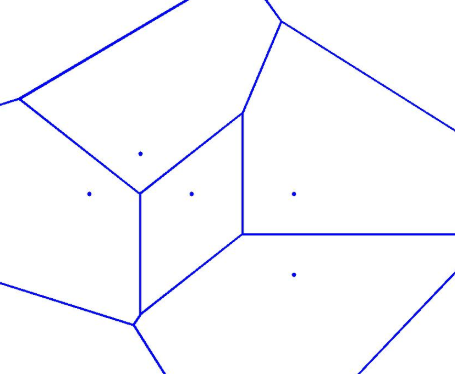
\includegraphics[width=0.3\textwidth]{voronoi.png}
\qquad\qquad
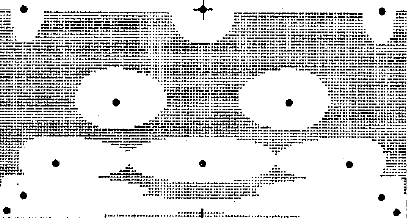
\includegraphics[width=0.35\textwidth]{Juang-cell_shape.png}

\begin{itemize}
    \item Partition the $P$-dimensional space into $M$ regions
         that "best" represent the predictor vectors
         arising from song units instances

    \item "Best" in terms of minimizing some overall distortion measure

    \item Let $\bC \equiv \langle C_1,C_2,\ldots,C_M \rangle$ be
        the set of centroids that best represent the space

\end{itemize}

}

\frame{
\frametitle{Vector Quantization}

\begin{itemize}
    \item \alert{Quantization}:\\
        With \bC, we can map each $\ba^{(t)}$ to a symbol $o_t$:
        \begin{equation*}
         o_t \gets \argmin\limits_{k=1}^{M} d(\ba^{(t)}, C_k)
        \end{equation*}

\end{itemize}

}

\frame{
\frametitle{Hidden Markov Model}

\begin{itemize}
    \item $\pi$, initial state probability distribution:
        \[
            \pi = (\pi_1, \pi_2, \ldots, \pi_N)
        \]

    \item  $A$, state transition distributions:
        \[
            A =
            \begin{bmatrix}
                a_{11} & a_{12} & \dots  & a_{1N} \\
                a_{21} & a_{22} & \dots  & a_{2N} \\
                \vdots & \vdots & \ddots & \vdots \\
                a_{N1} & a_{N2} & \dots  & a_{NN}
            \end{bmatrix}
        \]

    \item $B$, observation symbol distributions:
        \[
            B =
            \begin{bmatrix}
                b_{11} & b_{12} & \dots  & b_{1M} \\
                b_{21} & b_{22} & \dots  & b_{2M} \\
                \vdots & \vdots & \ddots & \vdots \\
                b_{N1} & b_{N2} & \dots  & b_{NM}
            \end{bmatrix}
        \]
\end{itemize}

}


\frame{
\frametitle{Hidden Markov Modeling}

\tikzset{every picture/.style={line width=0.75pt}} %set default line width to 0.75pt

\begin{tikzpicture}[x=0.75pt,y=0.75pt,yscale=-0.8,xscale=0.8]
    %uncomment if require: \path (0,425); %set diagram left start at 0, and has height of 425

    %Shape: Circle [id:dp023172788570489544]
    \draw   (41.33,126.33) .. controls (41.33,117.86) and (48.2,111) .. (56.67,111) .. controls (65.14,111) and (72,117.86) .. (72,126.33) .. controls (72,134.8) and (65.14,141.67) .. (56.67,141.67) .. controls (48.2,141.67) and (41.33,134.8) .. (41.33,126.33) -- cycle ;
    %Shape: Circle [id:dp5630020814965475]
    \draw   (131.33,126.33) .. controls (131.33,117.86) and (138.2,111) .. (146.67,111) .. controls (155.14,111) and (162,117.86) .. (162,126.33) .. controls (162,134.8) and (155.14,141.67) .. (146.67,141.67) .. controls (138.2,141.67) and (131.33,134.8) .. (131.33,126.33) -- cycle ;
    %Rounded Rect [id:dp19918097970232473]
    \draw   (35.33,190.27) .. controls (35.33,187.36) and (37.69,185) .. (40.6,185) -- (57.07,185) .. controls (59.98,185) and (62.33,187.36) .. (62.33,190.27) -- (62.33,206.07) .. controls (62.33,208.98) and (59.98,211.33) .. (57.07,211.33) -- (40.6,211.33) .. controls (37.69,211.33) and (35.33,208.98) .. (35.33,206.07) -- cycle ;
    %Rounded Rect [id:dp2970451840947941]
    \draw   (141.33,190.27) .. controls (141.33,187.36) and (143.69,185) .. (146.6,185) -- (163.07,185) .. controls (165.98,185) and (168.33,187.36) .. (168.33,190.27) -- (168.33,206.07) .. controls (168.33,208.98) and (165.98,211.33) .. (163.07,211.33) -- (146.6,211.33) .. controls (143.69,211.33) and (141.33,208.98) .. (141.33,206.07) -- cycle ;
    %Rounded Rect [id:dp9330541213547303]
    \draw   (86.33,190.27) .. controls (86.33,187.36) and (88.69,185) .. (91.6,185) -- (108.07,185) .. controls (110.98,185) and (113.33,187.36) .. (113.33,190.27) -- (113.33,206.07) .. controls (113.33,208.98) and (110.98,211.33) .. (108.07,211.33) -- (91.6,211.33) .. controls (88.69,211.33) and (86.33,208.98) .. (86.33,206.07) -- cycle ;
    %Straight Lines [id:da3963740483943028]
    \draw [color={rgb, 255:red, 155; green, 155; blue, 155 }  ,draw opacity=1 ]   (97.67,71.33) -- (65.58,111.77) ;
    \draw [shift={(64.33,113.33)}, rotate = 308.44] [color={rgb, 255:red, 155; green, 155; blue, 155 }  ,draw opacity=1 ][line width=0.75]    (10.93,-3.29) .. controls (6.95,-1.4) and (3.31,-0.3) .. (0,0) .. controls (3.31,0.3) and (6.95,1.4) .. (10.93,3.29)   ;

    %Straight Lines [id:da5589319927065257]
    \draw [color={rgb, 255:red, 155; green, 155; blue, 155 }  ,draw opacity=1 ]   (105,72) -- (137.08,111.78) ;
    \draw [shift={(138.33,113.33)}, rotate = 231.12] [color={rgb, 255:red, 155; green, 155; blue, 155 }  ,draw opacity=1 ][line width=0.75]    (10.93,-3.29) .. controls (6.95,-1.4) and (3.31,-0.3) .. (0,0) .. controls (3.31,0.3) and (6.95,1.4) .. (10.93,3.29)   ;

    %Curve Lines [id:da32985837578553223]
    \draw [color={rgb, 255:red, 155; green, 155; blue, 155 }  ,draw opacity=1 ]   (39.75,120) .. controls (13.67,121.71) and (17.29,135.53) .. (39.74,134.37) ;
    \draw [shift={(41.5,134.25)}, rotate = 535.24] [color={rgb, 255:red, 155; green, 155; blue, 155 }  ,draw opacity=1 ][line width=0.75]    (10.93,-3.29) .. controls (6.95,-1.4) and (3.31,-0.3) .. (0,0) .. controls (3.31,0.3) and (6.95,1.4) .. (10.93,3.29)   ;

    %Curve Lines [id:da05241887412967472]
    \draw [color={rgb, 255:red, 155; green, 155; blue, 155 }  ,draw opacity=1 ]   (163.25,119.5) .. controls (187.51,116.32) and (189.43,134.5) .. (163.38,134.05) ;
    \draw [shift={(161.75,134)}, rotate = 362.58000000000004] [color={rgb, 255:red, 155; green, 155; blue, 155 }  ,draw opacity=1 ][line width=0.75]    (10.93,-3.29) .. controls (6.95,-1.4) and (3.31,-0.3) .. (0,0) .. controls (3.31,0.3) and (6.95,1.4) .. (10.93,3.29)   ;

    %Curve Lines [id:da20868136012160865]
    \draw [color={rgb, 255:red, 155; green, 155; blue, 155 }  ,draw opacity=1 ]   (73,118) .. controls (100.74,107.39) and (112.89,110.27) .. (128.53,118.13) ;
    \draw [shift={(130.25,119)}, rotate = 207.26] [color={rgb, 255:red, 155; green, 155; blue, 155 }  ,draw opacity=1 ][line width=0.75]    (10.93,-3.29) .. controls (6.95,-1.4) and (3.31,-0.3) .. (0,0) .. controls (3.31,0.3) and (6.95,1.4) .. (10.93,3.29)   ;

    %Curve Lines [id:da40913443372744696]
    \draw [color={rgb, 255:red, 155; green, 155; blue, 155 }  ,draw opacity=1 ]   (131.75,134) .. controls (106.51,144.29) and (102.17,144.02) .. (72.59,133.18) ;
    \draw [shift={(70.75,132.5)}, rotate = 380.2] [color={rgb, 255:red, 155; green, 155; blue, 155 }  ,draw opacity=1 ][line width=0.75]    (10.93,-3.29) .. controls (6.95,-1.4) and (3.31,-0.3) .. (0,0) .. controls (3.31,0.3) and (6.95,1.4) .. (10.93,3.29)   ;

    %Straight Lines [id:da1317521888336055]
    \draw [color={rgb, 255:red, 155; green, 155; blue, 155 }  ,draw opacity=1 ]   (56.67,141.67) -- (45.55,180.58) ;
    \draw [shift={(45,182.5)}, rotate = 285.95] [color={rgb, 255:red, 155; green, 155; blue, 155 }  ,draw opacity=1 ][line width=0.75]    (10.93,-3.29) .. controls (6.95,-1.4) and (3.31,-0.3) .. (0,0) .. controls (3.31,0.3) and (6.95,1.4) .. (10.93,3.29)   ;

    %Straight Lines [id:da29906892694948883]
    \draw [color={rgb, 255:red, 155; green, 155; blue, 155 }  ,draw opacity=1 ]   (134.5,139.5) -- (65.97,179.98) ;
    \draw [shift={(64.25,181)}, rotate = 329.43] [color={rgb, 255:red, 155; green, 155; blue, 155 }  ,draw opacity=1 ][line width=0.75]    (10.93,-3.29) .. controls (6.95,-1.4) and (3.31,-0.3) .. (0,0) .. controls (3.31,0.3) and (6.95,1.4) .. (10.93,3.29)   ;

    %Straight Lines [id:da6190926392565461]
    \draw [color={rgb, 255:red, 155; green, 155; blue, 155 }  ,draw opacity=1 ]   (61.5,142.5) -- (98.12,181.05) ;
    \draw [shift={(99.5,182.5)}, rotate = 226.47] [color={rgb, 255:red, 155; green, 155; blue, 155 }  ,draw opacity=1 ][line width=0.75]    (10.93,-3.29) .. controls (6.95,-1.4) and (3.31,-0.3) .. (0,0) .. controls (3.31,0.3) and (6.95,1.4) .. (10.93,3.29)   ;

    %Straight Lines [id:da4382434052833961]
    \draw [color={rgb, 255:red, 155; green, 155; blue, 155 }  ,draw opacity=1 ]   (69,143) -- (143.72,181.58) ;
    \draw [shift={(145.5,182.5)}, rotate = 207.31] [color={rgb, 255:red, 155; green, 155; blue, 155 }  ,draw opacity=1 ][line width=0.75]    (10.93,-3.29) .. controls (6.95,-1.4) and (3.31,-0.3) .. (0,0) .. controls (3.31,0.3) and (6.95,1.4) .. (10.93,3.29)   ;

    %Straight Lines [id:da6400163637800176]
    \draw [color={rgb, 255:red, 155; green, 155; blue, 155 }  ,draw opacity=1 ]   (143.5,144) -- (102.97,181.15) ;
    \draw [shift={(101.5,182.5)}, rotate = 317.49] [color={rgb, 255:red, 155; green, 155; blue, 155 }  ,draw opacity=1 ][line width=0.75]    (10.93,-3.29) .. controls (6.95,-1.4) and (3.31,-0.3) .. (0,0) .. controls (3.31,0.3) and (6.95,1.4) .. (10.93,3.29)   ;

    %Straight Lines [id:da3288565770555445]
    \draw [color={rgb, 255:red, 155; green, 155; blue, 155 }  ,draw opacity=1 ]   (152,144.5) -- (153.42,180) ;
    \draw [shift={(153.5,182)}, rotate = 267.71] [color={rgb, 255:red, 155; green, 155; blue, 155 }  ,draw opacity=1 ][line width=0.75]    (10.93,-3.29) .. controls (6.95,-1.4) and (3.31,-0.3) .. (0,0) .. controls (3.31,0.3) and (6.95,1.4) .. (10.93,3.29)   ;

    %Shape: Circle [id:dp07875628504577792]
    \draw   (269.33,96.33) .. controls (269.33,89.11) and (275.19,83.25) .. (282.42,83.25) .. controls (289.64,83.25) and (295.5,89.11) .. (295.5,96.33) .. controls (295.5,103.56) and (289.64,109.42) .. (282.42,109.42) .. controls (275.19,109.42) and (269.33,103.56) .. (269.33,96.33) -- cycle ;
    %Shape: Circle [id:dp7485003300921682]
    \draw   (368.33,96.33) .. controls (368.33,89.11) and (374.19,83.25) .. (381.42,83.25) .. controls (388.64,83.25) and (394.5,89.11) .. (394.5,96.33) .. controls (394.5,103.56) and (388.64,109.42) .. (381.42,109.42) .. controls (374.19,109.42) and (368.33,103.56) .. (368.33,96.33) -- cycle ;
    %Shape: Circle [id:dp027749500298719365]
    \draw   (466.33,96.33) .. controls (466.33,89.11) and (472.19,83.25) .. (479.42,83.25) .. controls (486.64,83.25) and (492.5,89.11) .. (492.5,96.33) .. controls (492.5,103.56) and (486.64,109.42) .. (479.42,109.42) .. controls (472.19,109.42) and (466.33,103.56) .. (466.33,96.33) -- cycle ;
    %Rounded Rect [id:dp2534825050500533]
    \draw   (270.25,192.62) .. controls (270.25,190.07) and (272.32,188) .. (274.87,188) -- (288.72,188) .. controls (291.27,188) and (293.33,190.07) .. (293.33,192.62) -- (293.33,206.63) .. controls (293.33,209.18) and (291.27,211.25) .. (288.72,211.25) -- (274.87,211.25) .. controls (272.32,211.25) and (270.25,209.18) .. (270.25,206.63) -- cycle ;
    %Straight Lines [id:da07425430882168493]
    \draw    (394.5,96.33) -- (464.33,96.33) ;
    \draw [shift={(466.33,96.33)}, rotate = 180] [color={rgb, 255:red, 0; green, 0; blue, 0 }  ][line width=0.75]    (10.93,-3.29) .. controls (6.95,-1.4) and (3.31,-0.3) .. (0,0) .. controls (3.31,0.3) and (6.95,1.4) .. (10.93,3.29)   ;

    %Straight Lines [id:da17934625967557993]
    \draw    (217.5,96.33) -- (267.33,96.33) ;
    \draw [shift={(269.33,96.33)}, rotate = 180] [color={rgb, 255:red, 0; green, 0; blue, 0 }  ][line width=0.75]    (10.93,-3.29) .. controls (6.95,-1.4) and (3.31,-0.3) .. (0,0) .. controls (3.31,0.3) and (6.95,1.4) .. (10.93,3.29)   ;

    %Rounded Rect [id:dp8602684134694178]
    \draw   (369.25,192.62) .. controls (369.25,190.07) and (371.32,188) .. (373.87,188) -- (387.72,188) .. controls (390.27,188) and (392.33,190.07) .. (392.33,192.62) -- (392.33,206.63) .. controls (392.33,209.18) and (390.27,211.25) .. (387.72,211.25) -- (373.87,211.25) .. controls (371.32,211.25) and (369.25,209.18) .. (369.25,206.63) -- cycle ;
    %Rounded Rect [id:dp39149828948166765]
    \draw   (467.25,192.62) .. controls (467.25,190.07) and (469.32,188) .. (471.87,188) -- (485.72,188) .. controls (488.27,188) and (490.33,190.07) .. (490.33,192.62) -- (490.33,206.63) .. controls (490.33,209.18) and (488.27,211.25) .. (485.72,211.25) -- (471.87,211.25) .. controls (469.32,211.25) and (467.25,209.18) .. (467.25,206.63) -- cycle ;
    %Straight Lines [id:da8982730139590711]
    \draw    (479.42,110.42) -- (479.42,182.58) ;
    \draw [shift={(479.42,184.58)}, rotate = 270] [color={rgb, 255:red, 0; green, 0; blue, 0 }  ][line width=0.75]    (10.93,-3.29) .. controls (6.95,-1.4) and (3.31,-0.3) .. (0,0) .. controls (3.31,0.3) and (6.95,1.4) .. (10.93,3.29)   ;

    %Straight Lines [id:da8257412942305069]
    \draw    (295.5,96.33) -- (365.33,96.33) ;
    \draw [shift={(367.33,96.33)}, rotate = 180] [color={rgb, 255:red, 0; green, 0; blue, 0 }  ][line width=0.75]    (10.93,-3.29) .. controls (6.95,-1.4) and (3.31,-0.3) .. (0,0) .. controls (3.31,0.3) and (6.95,1.4) .. (10.93,3.29)   ;

    %Straight Lines [id:da6380311744143885]
    \draw    (381.42,110.42) -- (381.42,182.58) ;
    \draw [shift={(381.42,184.58)}, rotate = 270] [color={rgb, 255:red, 0; green, 0; blue, 0 }  ][line width=0.75]    (10.93,-3.29) .. controls (6.95,-1.4) and (3.31,-0.3) .. (0,0) .. controls (3.31,0.3) and (6.95,1.4) .. (10.93,3.29)   ;

    %Straight Lines [id:da4015609214611917]
    \draw    (282.42,110.42) -- (282.42,182.58) ;
    \draw [shift={(282.42,184.58)}, rotate = 270] [color={rgb, 255:red, 0; green, 0; blue, 0 }  ][line width=0.75]    (10.93,-3.29) .. controls (6.95,-1.4) and (3.31,-0.3) .. (0,0) .. controls (3.31,0.3) and (6.95,1.4) .. (10.93,3.29)   ;

    %Straight Lines [id:da2218606746919296]
    \draw  [dash pattern={on 0.84pt off 2.51pt}]  (203,154.5) -- (523.59,154.5) ;



    % Text Node
    \draw (56,125) node   {$s_{1}$};
    % Text Node
    \draw (146,125) node   {$s_{1}$};
    % Text Node
    \draw (101,60) node   {$\pi $};
    % Text Node
    \draw (50,196) node   {$v_{1}$};
    % Text Node
    \draw (156,196) node   {$v_{3}$};
    % Text Node
    \draw (101,196) node   {$v_{2}$};
    % Text Node
    \draw (283,95) node   {$q_{1}$};
    % Text Node
    \draw (382,95) node   {$q_{2}$};
    % Text Node
    \draw (480,95) node   {$q_{3}$};
    % Text Node
    \draw (283,198) node   {$o_{1}$};
    % Text Node
    \draw (243,83) node   {$\pi $};
    % Text Node
    \draw (382,198) node   {$o_{2}$};
    % Text Node
    \draw (480,198) node   {$o_{3}$};
    % Text Node
    \draw (464,130) node   {$b_{q_{3}}$};
    % Text Node
    \draw (429,82) node   {$a_{q_{2}}$};
    % Text Node
    \draw (329,82) node   {$a_{q_{1}}$};
    % Text Node
    \draw (365,130) node   {$b_{q_{2}}$};
    % Text Node
    \draw (266,130) node   {$b_{q_{1}}$};


\end{tikzpicture}


\begin{itemize}
    \setlength\itemsep{1em}
    \item $\bq = \langle q_1, q_2, \ldots, q_T \rangle$:
        hidden state sequence

    \item $\bo = \langle o_1, o_2, \ldots, o_T \rangle$:
        our acoustic signal
\end{itemize}

}

\frame{
\frametitle{HMM Operations}

With $\lambda = (\pi, A, B)$ denoting an HMM

\begin{itemize}
    \setlength\itemsep{1em}

	\item For given $\bo$ and $\lambda$,
        compute $P[\bo|\lambda]$

    \item For given $\bo$ and $\lambda$,
        estimate a most likely state sequence $\bq^*$

	\item Learn a model $\lambda^* \equiv (\pi^*, A^*, B^*)$\\
        such that $P[\bo|\lambda^*]$ is maximized for a given
		observation sequence $\bo$

\end{itemize}

}

\frame {
\frametitle{Statistical Pattern Classification}

\begin{itemize}
    \setlength\itemsep{1em}
    \item Vocabulary of $R$ song unit types:\\
    \begin{equation*}
        U = \{ u_1, u_2, \ldots, u_R \}
    \end{equation*}

    \item Assume we have a \alert{model} $h_r$ for each unit type $u_r$.\\
    We are interested in computing:
    \begin{equation*}
        P[h_r|\bx] \equiv \text{Probability of $h_r$ given \bx}
    \end{equation*}

    \item Classification of an observation sequence \bx\\
    is based on a \alert{maximum likelihood} model selection:
    \begin{equation*}
        h^* \equiv \argmax\limits_{h\in H} P[h|\bx]
    \end{equation*}
    where $H = \{ h_1, \ldots, h_R \}$.

\end{itemize}
}

\frame{
\frametitle{Maximum Likelihood model selection}

\begin{equation*}
    \arraycolsep=1.4pt\def\arraystretch{2.2}
    \begin{array}{rcll}
        h^* &\equiv& \argmax\limits_{h\in H} P[h|\bx] \\
        &=& \argmax\limits_{h\in H} \frac{P[\bx|h] P[h]}{P[\bx]}  & \qquad \text{(Bayes' theorem)}\\
        &=& \argmax\limits_{h\in H} P[\bx|h] P[h]                 & \qquad \text{($P[\bx]$ is constant wrt $h$)}\\
        &=& \argmax\limits_{h\in H} P[\bx|h]                      & \qquad \text{(Assuming models are equiprobable)}\\
    \end{array}
\end{equation*}
}



\end{document}
